\documentclass{article}
\usepackage{multicol}
\usepackage{fullpage}
\usepackage[english]{babel}
\usepackage{blindtext}
\usepackage{graphicx}
\addtolength{\oddsidemargin}{-0.4in}
\addtolength{\evensidemargin}{-0.3in}
\addtolength{\textwidth}{0.7in}
\addtolength{\topmargin}{-0.4in}
\addtolength{\textheight}{0.8in}
\begin{document}
\title {pheno2geno}
\author{
Konrad Zych\,$^{1,2}$, 
Danny Arends\,$^{2,}$,
 Ritsert C. Jansen\,$^{2}$
}
\maketitle
{\noindent}1. Faculty of Biochemistry, Biophysics and Biotechnology, Jagiellonian University in Krakow, Poland \\*
2. Groningen Bioinformatics Center, University of Groningen, The Netherlands

\newpage
\section{General introduction}
\begin{multicols}{2}
{\noindent}Genetical Genomics (citation) is powerful method, providing world of life sciences with tool to look deep inside the complex relation between genetic information stored by DNA and final outcome of its processing - phenotype. And because this is the core dogma of modern biology, every method helping us to understand it better is of high importance to scientific world. 

{\noindent}Great power often comes for high price, though. To perform GG studies one has to obtain both phenotypic and genotypic data, that are subsequently being matched. This not only elevates costs of experiment, but also introduces number of human errors, e.g. mismatching/mislabeling of arrays.

{\noindent}This brought us back to DNA to phenotype dogma. And we came up with idea of creating genetic map out of gene expression data. This means the same power for less then half of the cost and effort. Procedure is easy enough to be conducted by inexperienced R user and for advanced users we offer variety of extra functionalities to make their analysis fit their needs.
\subsection{R programming language}
R programming language is powerful, yet easy-to-use. There is graphical interface available for Windows, Mac OS and Linux. Every package/function comes with easily accessible help file and, most importantly, R provides user with handfuls of statistical functionalities. To start your adventure with R just go to: http://cran.r-project.org/, select your operating system, install it, and you're ready to enter the world of R.
\subsection{Downloading and installing package}
R packages contribute to power of this language more than anything. Using then, you can extend basic R to powerful tool perfectly suited to your personal needs. Installing package is really easy, just open R gui and type:
> install me
> or what?
or use Packages menu (just click on Install Packages, select a mirror and than select package pheno2geno).
\end{multicols}
\newpage
\section{Data}
\begin{multicols}{2}
\subsection{Data files' structure}
{\noindent}In order to ensure smooth work of our package, we specified strict rules about data files provided. If below mentioned requirements are met and filenames are default, user don't have to provide reading function with any parameters. If your more advanced R user, your data files are of different format or you have data already inside R environment, please see section 4.1. 
\subsubsection{Phenotype data for offspring}
This data is crucial and analysis cannot be run without it. Default filename is offspring\_phenotypes.txt. Rows correspond to markers and columns to individuals. File should contain only numeric values apart from first row, containing unique column names and first column containing unique row names. Rows and columns with non-numeric values are removed. All values should be separated by tabs. In normal practice first row has one element less then others (no column name for column containing rownames).
\subsubsection{Phenotype data for founders}
This data is optional but really important for the analysis, so we recommend to provide it. Default filename is founders\_phenotypes.txt. Data structure inside the file should be the same as in offspring phenotype file. Also row names should match, because non-matching rows are removed.
\subsubsection{Genotype data for offspring}
This data is optional and doesn't have any impact on analysis, could be only used for creating cross object out of existing data using our software. Default filename is offspring\_genotypes.txt. Genotypes should be coded as 0,1 and NA. Data structure inside the file should be the same as in offspring and founders phenotype files. Row names should match, because non-matching rows are removed. 
\subsubsection{Genetic map}
This data is optional and could be used for comparison with map created by our software or for ordering markers in output cross. Default filename is maps\_genetic.txt. File should contain three columns - marker name, chromosome number and position on chromosome in cM. Second and third column should contain numeric values without NAs, NaNs, etc. First column should contain unique marker names, matching ones in phenotype files.
\subsubsection{Physical map}
Exactly the same as in genetic map, but position on chromosome should be in Mbp.
\end{multicols}
\begin{multicols}{2}
\subsection{Population object}
To store all the necessary information and mainupulate it easily we developed object of class population (schematically shown on figure 1). It's divided in three main parts:
\begin{itemize}
\item  founders part, storing founders phenotype data, information about founders groups used by RankProduct analysis (see 3.2) and results of this analysis (RP object, futher documentation about it is available in help file of RP function),
\item  offspring part, storing founders phenotype and genotype data (read from file and/or simulated by our software),
\item maps part, storing genetic and/or physical map
\end{itemize}
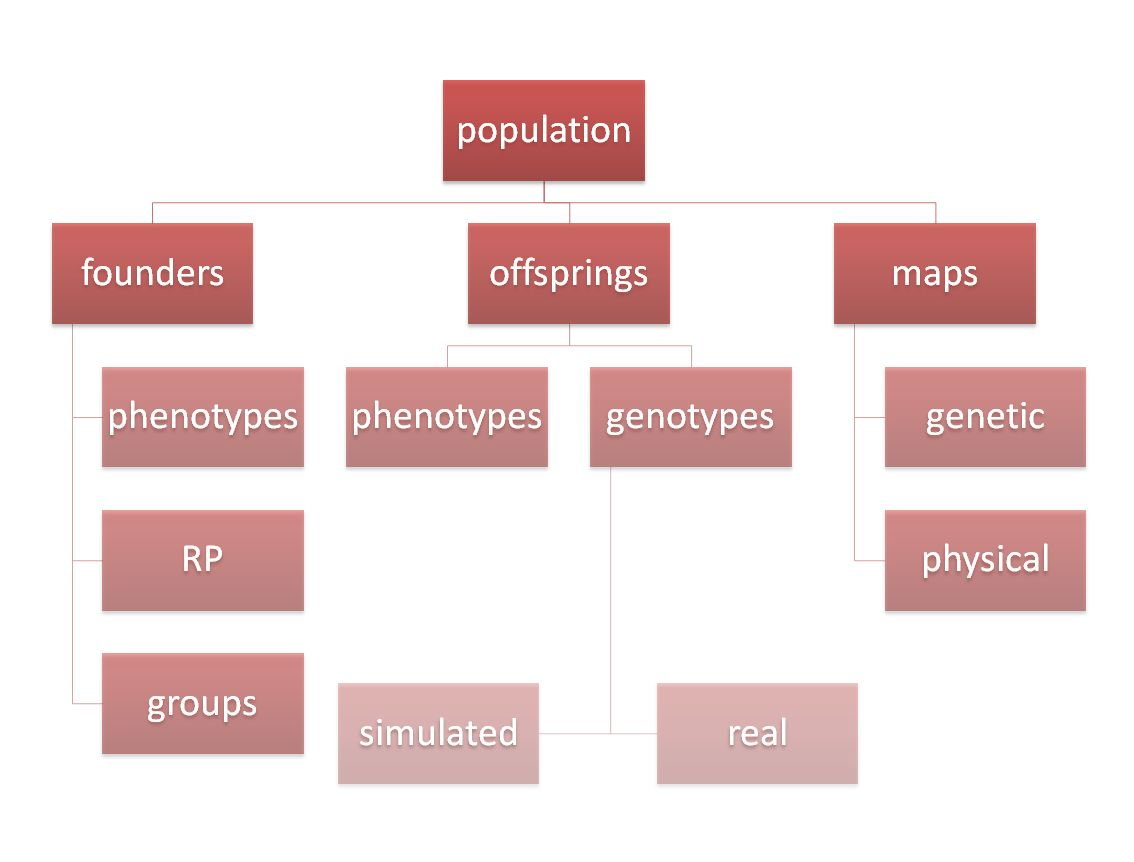
\includegraphics[scale=0.22]{population.jpg}
\end{multicols}
\newpage
\section{Basic workflow}
\begin{multicols}{2}
\subsection{Loading data into workflow}
If data is formatted as specified in chapter 2 and files are having default names, you just have to type: population <-  readFiles() into Rgui (make sure your working directory is the one containing data files) and it's all done. If you want to customize your files names, that can be done, but only to some extend. First of all you're able only to specify "cores": 
\begin{itemize}
\item  founders core, then name of the file containing founders phenotype data should be founders core\_phenotypes.txt
\item  offspring core,  then name of the file containing offspring phenotype data should be offspring core\_phenotypes.txt and file containing genotype data should be called offspring core\_genotypes.tx
\item maps core, then file maps core\_genetic.txt contains genetic map, while maps core\_physical.txt - physical map.
\end{itemize}
If you are more advanced in R and want to use your own data files of different names and/or structure, see section 4.1.
\subsection{Rank product analysis}
Rank Product (citation) is a powerful method for discovery of
 
\subsection{Preoptimized parameters for most common experimental crosses}
\blindtext
\subsection{Selecting appriopriate markers}
\blindtext
\subsection{Splitting selected markers}
\subsubsection{Parental mean splitting}
\blindtext
\subsubsection{EM splitting}
\blindtext
\subsection{Filtering markers}
\blindtext
\subsection{Cross object}
\blindtext
\subsubsection{Creating cross object}
\blindtext
\subsubsection{Forming linkage groups and \\* ordering markers}
\blindtext
\subsubsection{Augmenting cross object}
\blindtext
\end{multicols}
\newpage
\section{Advanced options/modifications}
\begin{multicols}{2}
\subsection{Using data files with different \\* structure}
\blindtext
\subsection{Rank product analysis}
\blindtext
\subsection{Uncommon types of crosses}
\blindtext
\subsection{Modifying splitting options}
\blindtext
\subsection{Filtering markers}
\blindtext
\subsection{Cross object}
\blindtext
\subsubsection{Forming linkage groups and \\* ordering markers}
\blindtext
\subsubsection{Post-processing of cross object}
\blindtext
\end{multicols}
\newpage
\section{Built-in plotting routines}
\subsection{plotChildrenExpression}
\blindtext[2]
\subsection{plotParentalExpression}
\blindtext[2]
\subsection{plotMapComparison}
\blindtext[2]
\subsection{plotMarkerDistribution}
\blindtext[2]
\newpage
\section{Big datasets}
\begin{multicols}{2}
\subsection{Problematic handling of big data by R}
\blindtext
\subsection{C preprocessing}
\blindtext
\subsection{Other solutions}
\blindtext
\end{multicols}
\newpage
\section{Package development \& collaboration}
\newpage
\section{References}
\end{document}